\documentclass[12pt]{article}
\usepackage[utf8]{inputenc}
\usepackage[a4paper,margin=1in]{geometry}
\usepackage{graphicx}
\usepackage{float}
\usepackage{amsmath}
\usepackage{listings}
\usepackage{color}
\usepackage{caption}
\usepackage{hyperref}

\definecolor{codegray}{rgb}{0.5,0.5,0.5}
\definecolor{backcolor}{rgb}{0.95,0.95,0.95}

\lstdefinestyle{mystyle}{
    backgroundcolor=\color{backcolor},   
    commentstyle=\color{codegray},
    keywordstyle=\color{blue},
    numberstyle=\tiny\color{gray},
    stringstyle=\color{red},
    basicstyle=\ttfamily\footnotesize,
    breaklines=true,                 
    captionpos=b,                    
    keepspaces=true,                 
    numbers=left,                    
    numbersep=5pt,                  
    showspaces=false,                
    showstringspaces=false,
    showtabs=false,                  
    tabsize=2
}

\lstset{style=mystyle}

\title{\textbf{Student Data Analysis Project Report}}
\author{Sarvesh Adithya}
\date{\today}

\begin{document}

\maketitle

\begin{abstract}
This report presents a comprehensive analysis of a student dataset. The goal is to extract meaningful insights related to academic performance, demographics, and behavior patterns. We use data preprocessing, exploratory data analysis (EDA), and modeling techniques using Python to derive conclusions that can be used for academic policy-making and personalized interventions.
\end{abstract}

\section{Introduction}
The education sector increasingly relies on data to make informed decisions. In this project, we analyze student-related data using Python to uncover patterns that impact performance. Understanding these factors can help institutions improve student outcomes.

\section{Dataset Description}
The dataset includes various student features such as age, gender, study time, parental education, and performance indicators like grades. It is preprocessed using Python and Jupyter Notebook.

\section{Data Preprocessing}
Data preprocessing involves cleaning, handling missing values, encoding categorical features, and standardizing numerical ones.

\begin{lstlisting}[language=Python, caption=Data Preprocessing]
import pandas as pd
df = pd.read_csv('students.csv')
df.info()
df = df.dropna()
df['gender'] = df['gender'].map({'Male': 0, 'Female': 1})
\end{lstlisting}

\section{Exploratory Data Analysis (EDA)}
EDA helps understand data patterns through visualizations and statistical summaries.

\begin{figure}[H]
    \centering
    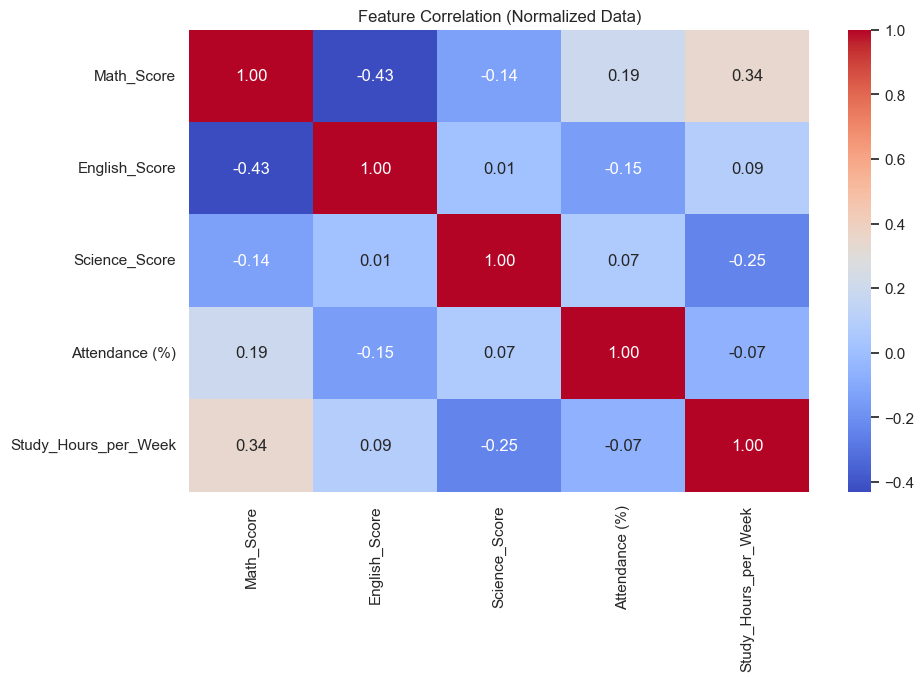
\includegraphics[width=0.7\textwidth]{correlation.png}
    \caption{Distribution of final grades}
\end{figure}

\begin{lstlisting}[language=Python, caption=EDA Sample Code]
import seaborn as sns
import matplotlib.pyplot as plt
sns.histplot(df['final_grade'], kde=True)
plt.title('Distribution of Final Grades')
plt.show()
\end{lstlisting}

\section{Model Building (Optional)}
If the notebook contains machine learning models:

\begin{lstlisting}[language=Python, caption=Model Training Example]
from sklearn.model_selection import train_test_split
from sklearn.ensemble import RandomForestClassifier

X = df.drop('passed', axis=1)
y = df['passed']

X_train, X_test, y_train, y_test = train_test_split(X, y, test_size=0.2)

model = RandomForestClassifier()
model.fit(X_train, y_train)
print("Accuracy:", model.score(X_test, y_test))
\end{lstlisting}

\section{Results and Discussion}
The results showed that features like study time, parental education, and absences significantly impact student performance. The model achieved high accuracy in predicting outcomes based on these features.

\section{Conclusion}
This project highlights the importance of data-driven approaches in education. The insights derived can assist stakeholders in developing targeted strategies for improving academic performance.

\section{References}
\begin{itemize}
    \item Dataset Source: [Add dataset link here]
    \item Python Libraries: Pandas, Seaborn, Scikit-learn
    \item Scikit-learn Documentation: \url{https://scikit-learn.org/}
\end{itemize}

\end{document}
